\chapter{Introduction}
This document is describing the Master Thesis developed by Manuel Pasieka as part
of the Master in Artificial Intelligence at UNIVERSIDAD INTERNACIONAL DE LA RIOJA, S.A.
2018-2019. \par

\bb

As part of the Thesis we developed an Agent-based simulation named
\textbf{Breakfastclub} (available at http://github.com/mapa17/breakfastclub) of
a virtual classroom in order to study the effect of different Personality Traits
on happiness and attention in a simulated class. This document is describing the
development of the project and the results achieved.

\bb

The document is split into the following chapters.
\begin{itemize}
\item This first chapter introduces the reader into the motivation behind this work and
its novelties.
\item The second chapter will discuss the state of the art of the methods and technologies
applied.
\item The third chapter lays out the initials objectives as well as their adaption
and final objectives of the Thesis.
\item The fourth chapter describes in detail the implementation and technical solution
to the proposed problem.
\item The fifth chapter is focused on the Data Analysis of the results generated.
\item The sixth chapter is providing a conclusion and summary of what has been
presented, as well as an outlook on possible future projects and extensions.
\end{itemize}

\section{Origin and Motivation}
The social climate of modern classrooms have been studied extensively in the past \cite{Anderson1982},
but common to many social studies, only the results of few empirical studies have been modeled
successfully. This is changing, and in part because of the availability of
computational methods and the availability of public data. Methods from statistical
physics are applied more and more successfully in studying complex social systems
(an extensive review on the topic can be found in \cite{Castellano2007}).

\bb

One method that has proven especially useful in studying social systems are
\textbf{agent-based models}\cite{Jackson2017} that are a special type of multi-agent systems
which models the behavior of individuals and can be used to study their interactions
and emerging social behavior.

\subsection{Simulations in the Social Sciences}
In their work \cite{gilbert2005simulation} the authors give a short history of
simulations in the social sciences. They explain different reasons why simulations
can be applied with different objectives,ranging from better understanding a social
system, to prediction, to substitute human experts, as training tools, entertainment
or as tools to for discovery and formalization of models.

\bb

Specially the later applications of simulations in the social sciences are interesting
to us, as traditional approaches to understand complex phenomena in the social sciences
have been focused on comparing the results of empirical studies to hypothesis
generated with theoretical models.

One of the difficulty with this approach are the increasing costs of such studies
in face of more and more complex models. The growing complexity and the degree of
freedom of these models, demand a equally growing sample size increasing costs and the
resources needed to generate results that can be used to verify and reject hypothesis
in order to improve the models.

\bb

Figure \ref{Cycle-TSE} demonstrates how simulations can be used to support
the discovery and improvements of new models and theories. Given a theoretical model
one can produce hypothesis that are used to situate a simulation, providing the initial
conditions and input parameters for the simulation. The simulation models is than
run to produce concrete predictions, that can be compared to experimental studies.
The overlap between the prediction and measured results is than used to form new
hypothesis that can be used to improve theory and future models.


\begin{figure}[H]
    \makebox[\textwidth][c]{%
    \begin{minipage}[t]{10cm}
        \centering
        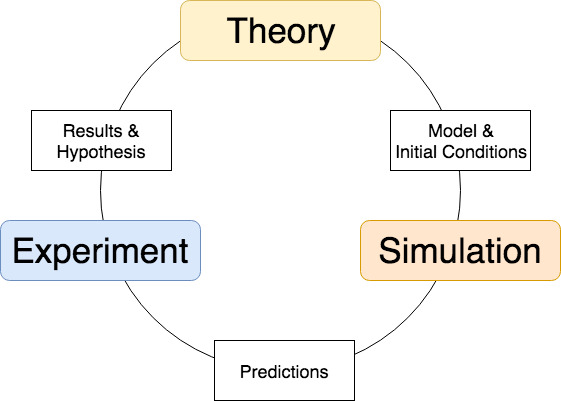
\includegraphics[width=300pt]{Theory-Simulation-Experiment}
        \caption{Cycle of Theory, Simulation and Experiment }
        \label{Cycle-TSE}
    \end{minipage}    
    }%
\end{figure}

\bb

As will be described in more detail later, our work is focused on studying the group
dynamics of children in a classroom, in particular that of a autonomous study group.

In order to achieve this, we split the task in two goals
\begin{enumerate}
    \item Develop a flexible and extendable agent-based model of a virtual classroom
    \item Study how different personality traits effect attention and happiness of individuals and the group as a whole
\end{enumerate}
